\documentclass[10pt,a4paper]{article}
\usepackage[utf8]{inputenc}
\usepackage[T1]{fontenc}
\usepackage{amsmath}
\usepackage{amsfonts}
\usepackage{amssymb}
\usepackage{graphicx}

\usepackage{comment}
\usepackage[ruled,vlined]{algorithm2e}

\author{Emma den Brok}
\title{A Systems Approach to Online Disinformation - One Year of Research}

\usepackage[natbibapa]{apacite}

\begin{document}
	\maketitle
	
	\tableofcontents
	
\section{Preface}
This document was written as a handover report for the research I did in one year for my PhD at TPM. It contains a motivation to apply a systems perspective to online disinformation, a literature review, and a proposal for a conceptual model of disinformation. If you have any questions about this report after reading, you can reach me at edenbrok@protonmail.com.

\section{Introduction}
\subsection{What is online disinformation?}
Online disinformation has been the topic of growing public and scientific interest. Speculation about the effect of online campaigns on the Brexit referendum, the Macron election and the US 2016 presidential election has been widespread. In the current COVID-19 pandemic, disinformation has also been a major source for concern, with the WHO stating it is an “infodemic” as much as a pandemic \cite{WHO2020}.  As a result of this public debate, there has also been more scientific attention for this topic. Empirical work on how exposure to (political) disinformation changes an individual’s belief has been limited and inconclusive thus far \citep{Tucker2018}. Some studies claim the effect of online disinformation campaigns was negligible in the outcome of the US election \citep{Allcott2017}, while others have found it can cause a shift in individuals beliefs \citep{Guess2020}. Anecdotal evidence does suggest that false information can have a major and potentially life-threatening effect on those who are exposed to it: Recently, hundreds of individuals in Iran were reported dead after they had ingested methanol, which had been falsely reported to cure COVID-19 \citep{Stone2020, Trew2020}. Western-Europe has seen multiple cases of fire being set to telecom masts, which are thought to be motivated by the belief that 5G is rolled out by governments in secrecy and is causing COVID-19 \citep{DeStandaard2020, Fildes2020, NOS2020}. \\

For a variety of disinformation examples, the goals with which it is spread directly relate to the falsehood of the information, for example when it is spread for political influence (i.e. false statements about a political opponent) \citep{keller2020political} or for monetary gain \citep{hrvckova2019unravelling}. However, sometimes the underlying goal of disinformation is not related to its content - for example when it is used to distract the public \citep{king2017chinese}. \cite{lewandowsky2017beyond} suggest that for this reason disinformation (which they refer to as \textit{post-truth claims}) should not just be treated as something poluting people's information environment, but as a political campaign with the goal of decreasing trust in institutions and true news. \cite{Starbird2019} uses the same logic to define \textit{strategic information operations} of which disinformation is a subset when the focusses is on spreading false messages or ideas rather than causing distraction or confusion. \\

In my research I did not scope to specific goals of disinformation as I believe a comprehensive, systems level understanding (more on this in Section \ref{systemsapproach}) of disinformation cannot disregard any of them. Because terminology across literature is often inconsistent yet overlapping, I provide two definitions here that I will use in the remainder of this document.\\ \\

\textit{\textbf{Disinformation} is false information that is knowingly and intentionally introduced into an information environment.} \\ \\

The focus is therefore on intent \citep{Fallis2015} and known (and hypothetically provable) falseness (following Kumar and Shah (2018)), therefore removing issues such as fake reviews out of the scope. This definition excludes \textit{misinformation} which is not introduced intentionally - though note that disinformation can still be spread or amplified by individuals who are unaware it is false once it is introduced in an information environment.

A piece of disinformation is seldomly spread in isolation - as \cite{Starbird2019} indicates they are often part of a larger operation with an underlying goal. Therefore, I also define disinformation campaigns: \\ \\

\textit{A \textbf{disinformation campaign} is a strategic effort by an actor to meet a specific goal by spreading (multiple pieces of) disinformation.} \\ \\

This emphasizes the fact that disinformation is often spread with a certain goal (monetary, political, social status, distraction) and that in order to meet this goal the actor who spreads disinformation has a pre-existing understanding or strategy of how disinformation can help them achieve that goal.



\subsection{Current strategies to address disinformation} \label{sec:strategies}
Though emperical work on the effect of disinformation remains inconclusive, the level of concern has lead to several stakeholders taking action. I briefly summarize the main strategies that are employed against online disinformation so far, focussing on governments and the tech sector. \\

\begin{figure}
	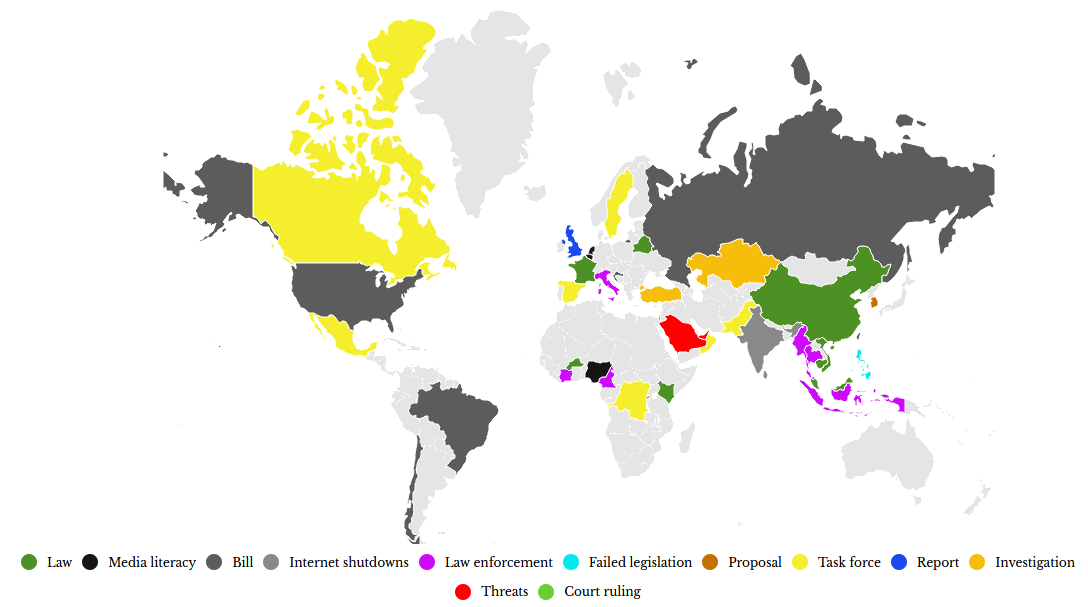
\includegraphics[scale=0.7]{govinitiatives.png}
	\caption{Approaches by governments across the globe. Map by Daniel Funke of Poynter (https://www.poynter.org/ifcn/anti-misinformation-actions)}
	\centering
	\label{img:govtresponse}
\end{figure}

A comprehensive overview of government responses to online mis- and disinformation is shown in Figure \ref{img:govtresponse}. The heterogeneity in responses is an indication of how governments are struggeling to address the issue. Moreover, in certain countries the laws or proposed bills include statements about ``false claims'' made about the government, showing how legal frameworks to tackle disinformation can be used for repression. Still, free-speech concerns are not exclusively relevant for repressive regiomes: In 2018, an EU anti-fake news initiative (EUvsDisinfo) drew criticism when it mislabelled three Dutch news websites as having posted disinformation \citep{Schenk2018}. Later, the EU adopted an initiative called the EU Action Plan Against Disinformation in spring 2019, which focussed on 4 pillars of response: 1) Improving their ability in detecting and analysing disinformation, 2) Strengthening joint responses, 3) Mobilising the private sector to address disinformation, and 4) Increasing societal resilience \cite{EuropeanCommission2018, kouroutakis2020eu}. The plan is seen as comprehensive and acknowledges the complexity of the problem, but suffers from the fact that the EU has limited legislative control over the US based online platforms. This makes it harder to enforce transparancy in the private sector, which plays an important role in the problem \citep{nenadic2019unpacking}. \\

In the U.S., several bills focussing on media literacy have passed on a state level and on a federal level a bill requiring transparancy on political ads was introduced \citep{Funke2020}. Still, a landscape analysis on actors addressing disinformation in the U.S. showed that most initiatives are lead by universities, media companies and foundations, and are funded by philanthropists rather than government or tech companies \citep{Legg2018}. After the Russian inteference in the 2016 U.S. election, tech companies have been under increased scrutiny to address the disinformation that is shared on their platforms. The reason why these platforms have only started to develop policies recently is that they fall under legistlation created in the the late 1990s which exempts them from liability of user content and behaviour \cite{bowers2020answering}. The recent surge in policies formulated by platform owners is seen as an attempt to avoid legislative changes in the US that would remove or reduce this exemption. \\\\

 The measures taken by these tech companies vary significantly across platforms. To highlight three: \textbf{Twitter} has completely banned political ads, stating that they believe political reach should be \textit{``earned, not bought''}\footnote{https://business.twitter.com/en/help/ads-policies/ads-content-policies/political-content.html}. Their policy when it comes to disinformation is to provide warnings in case content has been proven false or claims have been disputed, and to remove misinformation if its impact can be severly damaging\footnote{https://blog.twitter.com/en\_us/topics/product/2020/updating-our-approach-to-misleading-information.html}. \textbf{Facebook} has content fact-checked by third-party collaborators and provides labels if the content is misleading\footnote{https://www.facebook.com/facebookmedia/blog/working-to-stop-misinformation-and-false-news}. However, its approach to political ads is to not fact-check them at all, citing free speech concerns. There are rumors that Facebook might change its policy to also ban political ads \citep{Isaac2020NYT}. \textbf{Youtube} has policies to remove content which misleads voters (i.e. by advertising the wrong election date) as well as removing content that has been altered and can cause ``serious risk of egregious harm'' \citep{Miller2020YT}. It also claims to remove accounts associated with ``coordinated influence campaigns.'' It's approach to non-political dis- or misinformation is to surpress recommendations for this content, but it is not removed \citep{YT2019recom}. 



\subsection{Why we need a Systems Theory of Disinformation} \label{systemsapproach}
The responses to disinformation discussed in the previous sections were not only heterogeneous because it is unclear what approach is the most effective, but also because different elements that interact under the problem of disinformation are controlled by different actors. However, the properties of the content, how it spreads over a platform, the goals of the source, why it can become popular, why people believe it, how people end up in filter bubbles – all of these elements interact with each other in some way. Therefore, we should study all these elements in combination with each other - together they form the sociotechnical system in which disinformation takes place. \\

Sociotechnical systems are complex systems that consist both of technical artefacts and social components (i.e. people, institutions), that interact with and influence one another \citep{Nikolic2012}. The study of complex systems originates from systems theory, which was developed by Bertalanffy (amongst others \citep{Ryan2008}) to address the fact that many objects of study science is interested in cannot be studied in isolation, and that if a higher perspective is taken, the behaviour of the organisation of objects cannot be explained by the summation of the individual objects alone \citep{Bertalanffy1972}. Systems theory aims to find common aspects of these systems – the organisation of objects – across disciplines \citep{Boulding1956}. Complex systems science is one of the fields that evolved from the idea of systems theory which focuses on the exploration and explanation of emergent behaviour resulting from many different individual entities \citep{Ryan2008}. \\

Online disinformation is a typical example of a complex sociotechnical system: Its medium is digital technology, which it uses because of the social relationships and interactions that are formed using that technology. At the same time, the technology central to its succes is at the center of a highly contested political debate where the tug-of-war between governments and commercial platform owners is complicated by values such as privacy and freedom of speech. The interplay between the social and technical is everywhere: At the individual level, design choices made on these platforms influence how someone evaluates the content they see. On a societal level, there is an ongoing chicken-and-egg discussion about the direction of causality when it comes to social media use and polarisation. \\

Defining policies that tackle problems in sociotechnical systems is often considered a \textit{``wicked problem’’}: These are problems where it is unclear when they are solved, where testing solutions is hard and implementation of those solutions are essentially “one-shot operations”. Wicked problems are unique and – what really resonates with discourse on disinformation – can be seen as symptoms of another problem \citep{Rittel1973}. A similar perspective is taken in post-normal science, which  refers to the practice of science in contexts where uncertainty is high, there is no agreement on values, and decision-making involves both high stakes and time pressure. The idea of post-normal science was developed in the 1990s to address the position of science in these contexts, mainly from an environmental perspective. As I will show in the literature review, online disinformation has several typical post-normal properties. Most prominently, for various system elements and relationships, there are multiple plausible explanations of how they work. \\
%TODO: add refs for post-normal

Wicked, post-normal or complex - whatever label is put on the problem of online disinformation, one thing is clear: If we want to find succesful ways for addressing it, we need to consider the entire system in which online disinformation takes place - not just the isolated elements that make up the system. Obtaining a systems understanding of disinformation is the first step in trying to find solutions to stop disinformation. But we also need to acknowledge the ambiguity and uncertainty inherent in trying to describe such a system. In the literature review I will try to highlight this complexity and multitiude of explanations. This is followed by a proposal for a conceptual model (which, of course, is only one of the many possible conceptualisations and by no means the ``right'' one). 




\section{Literature Review}
In this section I review the existing literature on online disinformation as well as relevant work from adjacent fields such as network science, psychology of advertising and propeganda. \\

Since we are interested in exploring a systems perspective, I have created a classification of how disinformation can be studied from various system perspectives. The classification is built out of two dimensions: the dimension of disinformation that is studied, and the area of focus within the larger system discussed in the previous section.
Disinformation is usually studied in terms of:
\begin{itemize}
	\item The \textbf{content} of the campaign itself
	\item How it \textbf{spreads} in a system
	\item The \textbf{effect} it has in the system	
\end{itemize}
A systems perspective on disinformation can roughly be divided into four (overlapping and interacting) sub-elements:
\begin{itemize}
	\item \textbf{Technical infrastructure}: This includes both the physical as well as the digital infrastructure that makes up the internet, and more specifically, the websites and platforms on the internet which are used to spread disinformation and on which people are exposed to it.
	\item \textbf{Social infrastructure}: As we'll see in the literature review, disinformation is seldomly targeted to a single person: Instead, the relationships we form online and offline and the (group) identities we have also form a infrastructure which spreads (dis)information. 
	\item \textbf{Institutions}: As shown in Section \ref{sec:strategies} a variety of institutions play a role or have an interest in the system of disinformation, and power over the other system elements is divided between them.
	\item \textbf{Individual}: Of course, on the lowest level disinformation is noticed, read by, internalised and shared by individuals. 
\end{itemize}
The position of the various fields within this classification is shown in Figure \ref{img:litanalysis}. As we will see in the literature review, most fields only cover a few of these perspectives, and some combinations of dimensions and focus were not found in the literature I reviewed. Note that in reality, the borders in which a field operates are not as clear as the boxes in the figure suggests. \\

\begin{figure}
	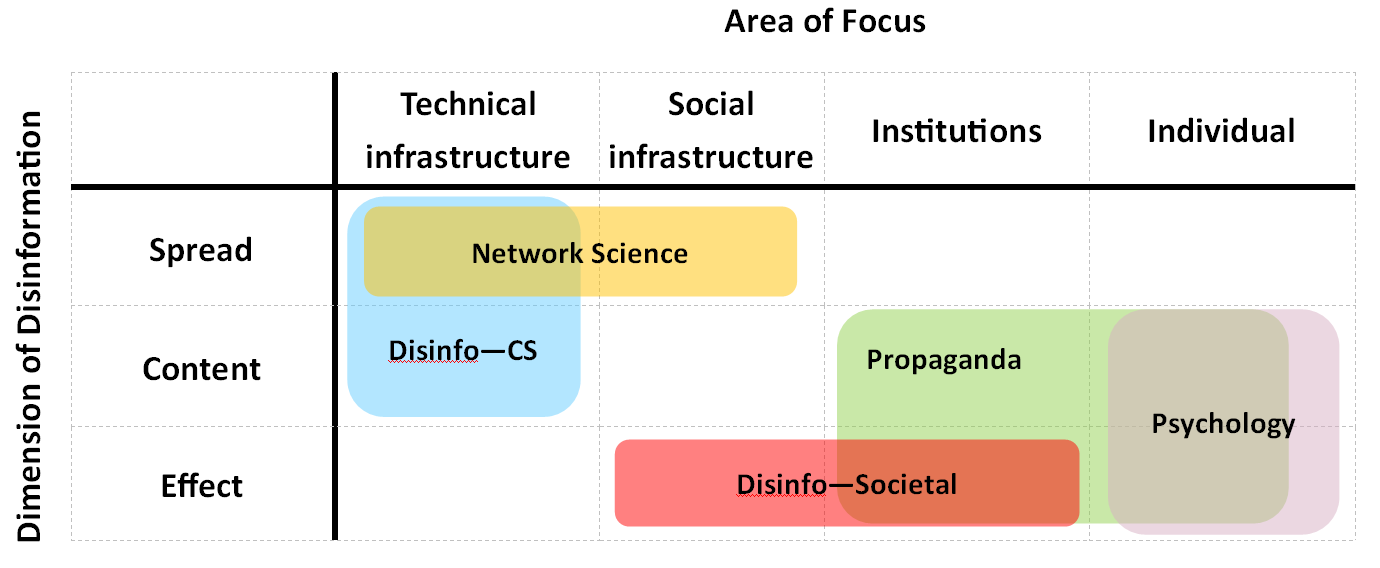
\includegraphics[scale=0.5]{litanalysis.png}
	\label{img:litanalysis}
	\caption{Classification of different research fields in terms of the dimension of disinformation and system elements they focus on. For research specifically about disinformation, I made a distinction between work based on computer/computational science (Disinfo - CS) and work focussing on the societal or poltical implications of disinformation (Disinfo - Societal)}
\end{figure}

\subsection{Disinformation Research}
In this section I provide a brief overview of disinformation research based on three perspectives:
\begin{itemize}
	\item \textbf{Computer Science:} The focus is on the detection of properties of disinformation, either of content itself (feature detection) or particular patterns of its engagement (i.e. likes, lifespan of interaction, spread over a network). 
	\item \textbf{Psychology:} Aims at understanding the psychological traits or mechanism that make individuals vulnerable to disinformation. 
	\item \textbf{Societal:} Discusses the effects disinformation has on a societal level, i.e. on politics, polarization, and behaviour.
\end{itemize}

\subsubsection{Computer Science Perspective}
The computer science perspective is motivated by the underlying assumption that if disinformation can be detected automatically it can be removed, surpressed or labeled before it reaches a large audience. One set of studies tries to identify features that allow them to predict whether a piece of content is false (or a rumour) or not. Such features may be content-based, network-based or platform specific  \citep{qazvinian2011rumor}, or based on the user who posted the content \citep{liu2015real}. Machine-learning approaches are also used to train algorithms on large annotated datasets (i.e. \cite{wang2017liar}, \cite{mitra2015credbank} \cite{papadopoulou2019corpus}) yet these approaches are labour-intensive and subsequent algorithms may be easily fooled and perform well only on the datasets they were trained on \citep{grondahl2018all}. \\

When studying how users engage with misinformation, \cite{Zollo2018} claim that the spread of misinformation is driven by confirmation bias and enabled by echo chambers that are formed on the web. The spread of the disinformation is therefore determined by the size of the echo chambers. \cite{DelVicario2016} also find that echo chambers play a role and find that the cascade behaviour of conspiracy theories is different than that of science stories.  \cite{Kumar2018} also see a role played by echo chambers, suggesting that the impact of disinformation is high when individuals see the same message repeated over and over, as would occur in echo chambers. However, in their review, \cite{Tucker2018} question the claim that echo-chambers play a central role, as other research has shown that users are exposed to a variety of viewpoints on online media. \cite{Vosoughi2018} consider only one type of content (news) and note that false news stories spread faster and further, and suggest this might be because they are more novel. They also find that bots spread both true and false news at similar rates, suggesting that the reach of false news is due to human behaviour. \cite{Budak2011} propose that looking at dynamics of spread can be the solution to stopping the spread of disinformation: if influential users can be “infected” with true information early on, this can halt the campaign. \\



\subsubsection{Psychological perspective}
Reviewing relevant literature, \cite{Kumar2018} provide three reasons why people are vulnerable to disinformation: People are unable to tell if information is false, particularly if it has been well-crafted, echo-chambers result in frequent exposure which increases belief, and mechanisms like confirmation bias, naïve realism and social norms lead people to seek confirmation of their own beliefs and the acceptance of peers. 

When it comes to an individual's ability to detect disinformation, \cite{Pennycook2018} found that people who have high ``bullshit receptivity'' and lower analytical thinking skills are more likely to perceive fake news as being accurate. \cite{uscinski2020people} Studied belief in COVID-19 related conspiracies, and found that belief in these was predicted by denialism, conspiracy thinking, and ideological motivations (i.e. Trump supporters were more likely to believe these conspiracies).

Related to the issue of echo-chambers and repeated information, \cite{Pennycook2018a}) found that the illusionary truth effect (statements seem more plausible when they are repeated) held for political disinformation, with a significant but small increase in perceived accuracy of fake news which participants had been exposed to previously. Notably, they showed that warnings that content was false did not decrease this effect. Closely related is the “continued influence effect” where people continue to rely on information they know to be false. Warnings and alternative explanations have been shown to reduce this effect, but cannot remove it completely \citep{Ecker2010}. \\


Two cognitive biases that likely play a role in the effect of disinformation are anchoring and confirmation bias. Anchoring is the process where the first data one receives strongly influences any future beliefs or estimates about the truth. \cite{jost2020fake} showed that this also occurs in the context of fake news, even when people are aware the information they receive is false Confirmation bias occurs when people are (unconsciouly) motivated to believe certain statements and reject others based on their previous beliefs. \cite{taber2006motivated} showed that in a political context, people are much more likely to accept arguments that support their previous beliefs and will pick apart counter-arguments. A similar process likely occurs with disinformation.

Little is know as of yet how these factors (personal skills, biases) are different across different contexts. \cite{Bessi2015} showed that on Facebook, people who were involved in conspiracy theories on one topic were more likely to be involved in other conspiracy theories as well. There is also some evidence that personal involvement increases the willingness of people to spread rumors, especially if they induce fear \citep{chua2018intentions}, suggesting that besides the topic, the ``stakes'' associated with disinformation can also influence how it is processed.



\subsubsection{Societal perspective}
Research on the subsequent effect of this exposure to the individual is limited. Based previous research on the effectiveness of political ads, \cite{Allcott2017}) claim that the exposure of disinformation based on a dataset of fake news about the 2016 US election had a negligible effect because the average American was only exposed to a handful of false stories. \cite{Guess2020} found that consumption of fake news was linked to distrust towards media and stronger feelings of polarisation. In additional experiments, they showed that a single exposure to a false story would increase the belief of the participant in the (political) claim made in that article. Though this change was significant it was also small, so it is not yet clear if there is a meaningful effect. \\ 

Disinformation may also work in less direct ways. For example, people may have wrong perceptions about public policy or events, and these may be encouraged by disinformation (i.e. exaggerating the money spent on welfare could be beneficial to the agenda of the Republican party.) \citep{Tucker2018}. \cite{Kolmes2011} argues that a lack of belief in man-made global warming in the American public was the result of disinformation that was deliberately spread by fossil fuel companies, but such a level of influence would be extremely hard to quantify. Indeed, the broader the perspective and the less defined the case, the harder it becomes to describe the effects of disinformation using emperical data. However, even if an effect is not immediately tangible, it does not mean it is absent.
\begin{comment}
if I wanted to go really wild I could talk about hyperobjects here but probably not the best place. Would be a nice concept to use later on though.
\end{comment}
\cite{Asmolov2018} believes that disinformation is effective not because of its actual content, but because the arguments it creates sever social ties, resulting in a polarized society. However, the direction of causality is not clear - some argue that the prevalence of echo chambers is exaggerated, and that polarization precedes large-scale online disinformation campaigns, which then make use of resulting biases (and possibly exaggerate them) \citep{Tucker2018}. Studying the interaction between the crowd and disinformation campaigns, \cite{Starbird2019} defines disinformation as a ``collaborative work:'' manipulation is not something that is done to a crowd, it is a process in which a crowd (unknowlingly) participates. They take the sociotechnical perspective, and using three case studies, show that the line between manipulator and user is not as clear as some of the platform policies aimed at detecting inauthentic behaviour would suggest. 
\cite{lewandowsky2017beyond} reject that with better communication techniques the issue of disinformation can be solved. In their work about the ``Post-Truth Era'' they identify a number of trends that they believe have contributed to the issue, ranging form a decrease in trust, growing inequality, polarization, and an (online) media landscape that rewards extremism. They state \textit{``...post-truth claims [...] do not seek to establish a coherent model of reality. Rather, they erode trust in facts and reality, to the point where facts no longer matter or are not even acknowledged to exist.''}.  \\

Based on this brief review, we can make a number of observations. The first is that efforts aimed at detecting and removing disinformation would need to focus on doing so almost immediately once a piece of disinformation is introduced into an online environment, since the psychological perspective suggests that warnings or removal at a later stage would be unsuccesful. This is already challenging, since actors who deliberately spread disinformation can change their tactics to avoid detection. But even assuming that detection is feasible, mass deletion of posts might have other risks. Given that individuals who are most likely to believe in disinformation are also distrusting towards media and authority, this could also create an effect where these groups move to other (less-controlled) platforms. 
Another observation is that polarization and echo-chambers are likely related to the succes of disinformation, but the direction and srength of this relationship remains up for debate. This is closely related to the outstanding issue of long-term effects of disinformation campaigns, which are hard to study emperically and occur in a wide context of social, politcal and economical factors that may all determine the effect of disinformation. The fact that these mechanisms remain unclear, combined with the current knowledge on what individuals are vulnerable to disinformation, suggest that a broader, societal perspective on disinformation is needed.


\subsection{Network Science}
\subsubsection{Why is network science relevant to disinformation?}
Online disinformation raises concern because it can be spread fast and far. This is due to two reasons: 1) Individuals can (unknowingly) act as amplefiers of content in their social circle, by easily sharing content with their connections or by drawing attention to it, and 2) the physical and digital infrastructure of the internet enables and encourages a number and span of connections that was not possible before. In this sense, online disinformation campaigns harness the social and digital infrastructure of the internet to their benefit. Both the social and digital infrastrucutres are \textit{networks}, which motivates this review of network science. Additionally, network science has long been used to study topics closely aligned with the problem of disinformation, such as the diffusion of information over a population and the rise (and fall) of political movements \citep{Guilbeault2018}. In the network science approach, a system is modelled as a collection of nodes and edges. Nodes are the object of interests (such as individuals or computers) and the edges indicate a connection between the nodes. The underlying assumption of network science is that these connections are fundamental in understanding the system of interest as a whole \citep{Brandes2013}.  \\

A key feature of many real-world networks is that they are not random – which means that there is something driving the formation of networks, and in turn, the formation of a network can be used to achieve certain aims \citep{Newman2003}. An important discovery in network science was that of the small-world model by \cite{Watts1998}, who showed that this network structure occurs in many real-world networks and demonstrated that diseases spread much faster over these networks. Small-world networks can mathematically be described as having a mean shortest distance between nodes that scales logarithmically or slower with the number of nodes N \citep{Newman2003}. 
\cite{Barabasi1999} found many real-world networks to have a degree distribution that followed a power-law distribution and called these networks scale-free networks. They showed that these types of network are created if networks are grown following preferential attachment: new nodes attach to nodes which already have a high number of edges.


\subsubsection{Information Diffusion, (Complex) Contagion and Network Strucutres}
As shown above, several different types of networks exist, influenced by the contexts in which they grew. Nowadays, many of the networks used daily are not grown organically – they are at least partly designed. Therefore, it is relevant to consider if design choices influence information diffusion – a highly relevant process when studying disinformation. I consider two types of network characteristics. Structural characteristics relate to the network properties discussed above, such as the distribution of node degrees and the average path length. Node characteristics relate to what behaviour a node can perform, i.e. how many neighbours it can communicate to at one time, the maximum number of connections it can maintain, or when it will form or break a connection. \\

The structure of a network has effects on how information, or a message, is propagated over it. \cite{Bampo2008} studied the effect of network topology on the success of a viral marketing campaign by simulating it over a random, small-world and scale-free network. The scale-free network was more sensitive to changes in the seed size and the average number of connections a message was passed on to.  \\

Some insight on the influence of node attributes can be gained from a marketing study, which showed that the spread of a Facebook application differed significantly depending on whether users could personally invite their friends, or if the application sent out passive notifications \cite{Aral2011}. Though personal invitations had a higher adoption rate, passive notifications were sent far more often and as a result, were more effective. Therefore, how a node can behave in a network influences diffusion. This also concerns how a node became active in the diffusion process in the first place, or how contagion works. \\

Long before network science appeared as a stand-alone discipline, sociologist \cite{Granovetter1977} showed that weak ties – edges that connect individuals who otherwise have little in common – greatly increase the reach and speed of information spreading over a network. This finding was later confirmed by the small-world model of \cite{Watts1998}. This so called “Strength of Weak Ties” explains why information and diseases can spread rapidly across the world – one edge is enough to link a group that is otherwise isolated from another. \cite{Centola2007} argued, however, that the strength of weak ties is dependent on what exactly is being diffused in the network. They showed that when considering complex contagion, where an individual needs to be exposed to multiple sources before being “activated” themselves, weak ties can lower diffusion. Whereas certain types of information or diseases can be passed on by a single moment of contact (simple contagion), more complex behaviours or beliefs may only be adopted once an individual sees that multiple of its connections have done so. As a result, on the same network, the pattern and size of diffusion differs depending on whether its spread is governed by simple or complex contagion.

\subsubsection{Multiplex networks} \label{sec:multiplex}
The literature discussed so far concerns properties of a single network. However, individuals seldomly partake in only one network. Multiple networks that are related to each other can be described through multiplex networks. Multiplex networks are networks where nodes are linked to each other with more than one type of edge, and the edges of one type that connect nodes together form one layer \citep{Lee2015}. Multiplex networks are of interest because interaction between the different layers can create non-additive and non-linear effects on the overall network. This is also why it is important to use multiplex networks when exploring systems that include multiple types of connections in reality – if the corresponding network model only has one layer, it may not correctly describe the behaviour of the system it should represent \citep{Lee2015}. \\

A property of interest in multiplex networks, which does not exist in single-layer networks, is the correlation between different layers. Correlation can be described in multiple ways, ranging from the extent of node multiplicity (i.e. how many vertices appear in different layers), to interlayer degree correlation, edge overlap, and cross-layered clustering coefficients \citep{Lee2015}. \\

In terms of diffusion over networks, it has been shown by \cite{Brummitt2012} in a case of threshold activation (a form of complex contagion, i.e. x number of neighbours need to be activated for a node to be activated), multiplex networks can show cascade effects even if the individual layers are not susceptible to global cascades. This shows that when studying cascade effects, it is necessary to consider any multiplicity in the system of interest. The same authors later showed that heterogeneity in threshold activation rules can enhance or inhibit cascades, depending on how many nodes require the threshold to be met in all layers \citep{Lee2014}. \cite{Sahneh2014}) showed that, when considering the diffusion of competing and exclusive viruses, in a multiplex network there exists an equilibrium in which the two viruses coexist simultaneously. In a single-layer network this is not possible: one of the two will always come to fully dominate the other. \\

\cite{Yagan2012} consider the case where the influence of two types of connections is weighted (i.e. the influence of a neighbour in one network is greater than that in the other) and analyse how this influences complex (threshold) contagion.  Their result show that both average degree and the relative difference in weighted influence strongly affect the probability of a global cascade, as well as its subsequent size. \\

The fact that network multiplicity has such a strong effect on probability and size of cascades has substantial consequences for studying the effect of disinformation. Most studies on the spread of disinformation (or closely related phenomena), model the spread of beliefs over a single layer network. However, individuals gain information from multiple sources and in the case of online disinformation, are likely exposed to mediating (or amplifying) influences from their offline (“real”) network of family and friends. Therefore, I propose that in order to properly study the spread of disinformation over a network, one needs to consider a multiplex network of at least two layers representing the online network and the offline network. 


\subsection{Psychology of advertising}
\cite{Fennis2015} define advertising as “any form of paid communication by an identified sponsor aimed to inform and/or persuade target audiences about an organization, product, service or idea.” Until the 20th century, advertisements focussed on the use of information or arguments to convince potential customers. In the early 1900s, advertisements also began using emotional appeals and the projection of ideas and beliefs. Both approaches have coexisted since then. \\

The psychology of advertising aims to identify how (characteristics) of advertisements affect individuals and to understand the psychological processes behind those effects \citep{Fennis2015}. The field was pioneered by \cite{Scott1916} with his book “The Psychology of Advertising”. Generally, three types of outcomes are studied: cognitive responses (beliefs and thoughts about a brand), affective responses (moods and emotions), and behavioural responses (buying a product, switching to a different brand) \citep{Fennis2015}. \\

Advertisers are mainly interested in changing the attitudes (which are made up of both cognitive beliefs as well as the affective state) of potential customers, as well as ensuring that a certain attitude leads to the desired behaviour. There are several theories on how attitudes change. One of the earliest was the Yale Attitude Change approach, developed by \cite{Hovland1953}, which focused on factors related to the source, the form of communication, and the audience. They also proposed several stages in which a message was processed, a framework that was extended in the Information Processing Model of \cite{McGuire1968}. He suggested six stages in which a message is processed: presentation, attention, comprehension, yielding, retention and behaviour. The stage of yielding is where attitude change occurs. Both the Yale Attitude Change model and the Information Processing Model assume that this is an active and conscious process. A different theory was proposed by \cite{Greenwald1968} in his Cognitive Response Model. He shifted away from models of learning and memorization of new information and stated that persuasion depended mainly on whether someone accepts the premise of the message when viewing it. \\

Dual process theories were developed to address the fact that the variables suggested by earlier models could not consistently explain the response to a message \cite{Xu2017}. The two prominent dual process models are the Elaboration Likelihood Model by Petty \& Cacioppo (1986) and the Heuristic Systematic Model by Chaiken et al (1980). In general these models assume that persuasion can happen in two ways: The first is through a conscious process in which the recipient engages with new information and adjusts their beliefs accordingly. The second route is reliant on heuristics and is used when someone’s motivation or skills are too low to process the information fully. Building on the dual process theories, \cite{Kruglanski1999} proposed the unimodel, suggesting that the two types of processing were not separate  processes, but variations of the same process that could be triggered by different contextual factors. \\

Advertisers are not only interested in convincing customers that their product is good, but hope that this is also translated in the behaviour of the customer. For a long time, attitude was seen as the most important predictor of behaviour. However, empirical studies showed that it could not be the sole explanation \citep{Fennis2015}. Fishbein and Ajzen formulated the Theory of Reasoned Action in the 1970s, which also took “subjective norms” into account (which describe social norms and the desire to comply with those norms by (not) performing a certain behaviour). They later extended this into the Theory of Planned Behaviour, which added the “perceived behavioural control” individuals had over the action they may perform (Ajzen, 1991). The three elements (attitude, subjective norm, and perceived behavioural control) predict the intention to perform a certain behaviour well, but there still remains a gap between intention and performing the behaviour itself \citep{Fennis2015}. \\

This theory, again, is based on a conscious process in which an intention is formed. Yet advertisers may also be interested in processes where certain behaviour is performed automatically.  The simplest form of this is habitual behaviour, where past behaviour is a better predictor than someone’s intention. However, advertisers may also try to prime behaviours to meet some goal (i.e. unconsciously smelling cleaning product might lead someone to formulate the goal of cleaning their house) \citep{Fennis2015}.  


\subsection{Propaganda} 
The Oxford English Dictionary defines propaganda as `` The systematic dissemination of information, esp. in a biased or misleading way, in order to promote a political cause or point of view.’’ \citep{OEDprop}. Propaganda was first studied in 500 BC in Athens through the lens of rhetoric. Non-western examples of propaganda from antiquity are the Artha-shastra (“The Science of Material Gain”) in India in 400 BC, and The Art of War by Sunzi \citep{Brittanica2020}. \\

The modern age of propaganda began at the start of the 20th century. Gustave Le Bon wrote a book in 1895 called “The Crowd: A Study of the Popular Mind” (in the then-new field of group psychology) which described techniques for propaganda (which were later adopted by Hitler). In the US, The Creel Commission was founded to develop a campaign to get the US involved in the first world war. Edward Bernays, who worked in this commission, coined the terms ``group mind’’ and` `engineering consent’’ \citep{Kim2007}. Harold D Lasswell published “Propaganda Technique in the World War” in 1927 and started the hype on analysing propaganda campaigns. This resulted in extensive employment of propaganda by governments and political movements during WWII and the Cold War to produce propaganda \citep{Brittanica2020}, the most infamous of which is probably Goebbles’ ministry of propaganda. \\

The most recent well-known theory of propaganda was defined by Herman and Chomsky in their 1988 book Manufacturing Consent. Their theory states that mass media fabricates consent for policies by their biases (or filters) in reporting. The five filters are: 1) The ownership of mass media by powerful, profit-oriented corporations, 2) The catering to existent economic desires by the media’s reliance on advertising for income, 3) The pressure to keep good relationships with (government) sources in order to maintain access to them, 4) ``Flack’’ (i.e. complaints, lawsuits) thrown at media by those who do not wish to be reported on, which drains the resources of the media, and 5) A narrative that exploits the fear of a common enemy. \\

A model of propaganda aligns well with most readings of disinformation is provided by \cite{ ross2002understanding}, who defines propaganda in terms of a sender, receiver and a message, with the core condition that propaganda has the goal to persuade. Ross stresses that the intent to persuade is not the same as an intent to lie. Propaganda messages are what she calls epistemically defective: They could be false, or badly argumented or reliant on emotional response. Moving away from the more restrictive definition of Hans Speier (a propaganda specialist working in the US during the second world war) and Herman and Chomsky, she says that propaganda does not have to come from (government) power; however, it does need to come from a political institution. Moreover, it needs to be aimed at a ``socially significant group’’ – that is, not just at a single individual. \\




\subsection{Research Gap}
On the basis of my literature review I've formulated the following research gaps:
\begin{itemize}
	\item \textbf{Dependence on scope \& contextual factors:} Psychological studies showed that individual beliefs and skills impact if people fall for disinformation, network studies show that the inclusion of multiple networks can change diffusion behaviour and even enable information cascades where they were not possible, and a simulation study found that changing the assumptions on how people share opinions determines the outcomes on a system level. Yet most literature does not (explicitly) address this dependence on context and sensitivity to scoping when it comes to disinformation. 
	\item \textbf{A variety of plausible (theoretical) explanations:} Explanations of why disinformation is so dangerous range from individual skills in media literacy, psychological biases we are all subject to, to features of the online platforms over which it is spread (i.e. bots, algorithms that encourage extremism), to broader social and economic trends such as a lack of trust in institutions and (economic) inequality. Relating to the previous point, which explanation is most appropriate is likely dependent on context. There is, however, no comprehensive work to explain what this variety of explanations means when trying to understand the problem on online disinformation.
	\item \textbf{Lack of a system-level, multidisciplinary/transdisciplinary approach:} The previous two points also strongly relate to this observation: There is very little work that tries to comprehensively bring together work on disinformation from various disciplines to understand how we may understand the problem on a system level (papers that do this are \cite{lewandowsky2017beyond} and \cite{Starbird2019}).
\end{itemize}


\section{Conceptual Model}

\subsection{Overview}
The \textbf{goal} of the conceptual model I describe here is theoretical exposition \citep{Edmonds2017} of a systems approach to online disinformation. That is, to explore the interaction between various system elements and to study the effect of contextual factors as well as different hypotheses on the functioning of subelements. The model should be able to represent real cases on a qualitative level (i.e. show the same dynamics or emergent behaviour) but is not meant to be predictive or be an exact quantitative representation of existing systems. \\

It follows from the preceding discussion that a model of disinformation should at least be able to represent the different areas the system consists of: The technical infrastructure of the online networks, the social infrastructure that represents relations between people, the institutions that send out (dis)information or want to tackle it, and the individual people who are affected by it. In this section I will describe a conceptual model for an ABM of online disinformation. The most important agents are individuals (people) who are connected to each other via networks over which they share information. They have internal states that describe their beliefs. Strategic actors (i.e. the spreader of disinformation, and institutions such as the platform owner or government) are not represented as agents but through underlying functions that observe and make changes to the networks (i.e. adding agents with certain beliefs or removing them).  \\

A factor that makes defining the conceptual model more complicated is the different goals actors who spread disinformation have. I believe it's still possible to define a general conceptual model of online disinformation, that can be adapted to represent different goals (i.e. beliefs, confusion, distraction) by changing the conceptualisation of the ``unit of flow'' of the model, which is always \textbf{information}. Throughout this conceptualization I will use the word ``belief'' to represent information, as information ``exists'' in the model as internal states of agents, who can then share their beliefs with others. Modelling these internal states in different ways (i.e. as continious scales, or as categorical states with an associated level of confidence) allows us to adapt the model to different goals. I will discuss this in more detail in Section \ref{beliefs}. \\

Structurally, the model is made up of two networks, one of which represents the ``real-life'' social network and one that represents the online platform (theoretically, you could expand to as many networks as you'd like to represent various online and offline communities and the overlap between them).\\

It is a conscious choice to model the online and offline networks as separate (but partly overlapping) networks. The relevant ABM studies I've seen (i.e. \cite{Ross2019} or \cite{Deffuant2002}) use only one network layer to represent a population of individuals whose opinion (or expression thereof) is influenced by others in the network. However, we know from network science (see Section \ref{sec:multiplex}) that network multiplicity can completly change cascade dynamics - exactly the thing spreaders of disinfo are interested in causing (and that we'd like to stop). In other words: When you talk to your friends, your newfound belief about lizard people ruling the earth might be challenged, and our model needs to account for that mediation. Fortunately, most people don't live solely in crazy Facebook groups. \\ 

\subsection{Agents and Actors}
The nodes (\textbf{agents}) of the networks are \textbf{individuals} or (only in the online network) \textbf{bots}.  \\

\textbf{Individuals} are agents that represent real people who shape their beliefs based on the information they receive from their network. In that sense this model assumes the social formation of beliefs - individuals do not evaluate the quality of the information or if it is consistent with their existing knowledge. That means the conceptual model is mainly suitable for context where the information is novel or subjective. 
Individuals have confidence in their beliefs, which can be used (in combination with other factors that depend on the way beliefs are modelled) to determine how likely they are to share their belief with their network. If their confidence is low, they may keep silent. Likewise, the belief along with their confidence in it can be used to break ties and form new ones. An individual may break a tie with someone if that person has shared a belief they strongly oppose - and will so so more easily in the online network. Likewise, an inidivudal may form new ties to find like-minded individuals. Sharing a belief and breaking and forming ties are the main actions that individuals take, but they do not have an overreaching goal they are working towards. \\

\textbf{Bots} is used as an umbrella term for any agent that is under control of a strategic actor (see below). In reality, these could be bots, trolls, fake accounts, or targeted advertisements. They do not evalute the beliefs they observe from their connections - instead, they will always post the belief that the spreading actor wants to promote. The internal structure of the bots is different, but other individuals are unable to distinguish between individuals and bots. It used to be fairly trivial to spot bots or trolls, but recently they have become increasingly convincing and in some cases go to great lengths to integrate into the target communities \citep{Starbird2019}. \\

Externally, both types of agents perform the same action: They broadcast their belief to their connections. The number of connections they can reach each timestep differs per network: The simpelest conceptualisation would be 1 connection in the offline network and all of the connections in the online network. For simplicity I also assume links in both networks are bidirectional. In reality, this would differ per social network and the ease with which bidirectional links can be established probably significantly affects how succesful bots or astroturf campaigns are. \\

The model also incorporates other \textbf{actors}, though not by modelling them as agents. These are actors are what I call ``strategic'' actors, in the sense that they observe what is happening in the simulation model and use their respective ``policy levers'' during runtime to change the model (i.e. adding or removing bots, promoting certain beliefs). \\

At the simplest level, there are three actors: the spreader, the platform owner, and a government (or any institution that will try to counter the disinformation campaign carried out by the spreader). The \textbf{spreader} is the actor who conducts the disinformation strategy to reach their goal using a specific \textit{strategy} to spread a belief. Their main resource is bots, but their strategy dictates how they are used - when they are activated, who they target, if all bots post the same belief etc. The \textbf{platform owner} is under pressure to tackle disinformation and does so by trying to detect bots. Though single individuals are unable to distinguish bots from genuine users, I assume platform owners are able to do so for the bots controlled by the spreader, by structurally analysing user behaviour (for an example of how this works, see \cite{beutel2013copycatch}). Social media platforms regularly announce they've removed large groups of accounts that were linked to suspicious activity. In the model, a platform owner can discover a group of bots that broadcasts the same belief with a probability dependent on the number of bots in the group. If they are detected they will be deleted. \\

Finally, the \textbf{government} (or countering actor) has an interest in the polulation holding a certain belief\footnote{If we're feeling optimistic, this would be a belief that's equivalent to the truth.}. Like the platforms, they can detect suspicious activity if a certain percentage of the nodes (individuals and bots) are sharing a contrary belief. In response, they can launch a counter-strategy. In contrast to the bots used by the spreader, I assume that individuals are able to identify posts that come from the government. This allows the model to incorporate decreased trust in (government) instutions. \\

It's unrealistic to assume that either the spreader or the government can employ an unlimited number of bots. The model should include a ``bot budget'' that limits the number of bots an actor can employ at one time. In terms of the strategies, there are many different possibilities. Bots could be set to target the most central individuals (preferential attachment), be spread randomly, or target specific clusters in the network. If strategic users do not use their budget in one timestep, the variations in strategies increase even further. 

\subsection{Conceptualisation of beliefs} \label{beliefs}
If the model is used to model a single statement that individuals can agree or disagree with, or two opposing statements, a continious scale is the simpelest conceptualisation (see Figure \ref{img:beliefs} on the left). For example, the statement could be "Climate change is man-made", or the opposing statements could be ``Yellow is the best color'' vs. ``Blue is the best color''. In this conceptualisation, both ends of the scale represent the extreme/strongest position, and the middle of the scale is the indifferent position. Individiuals shift their beliefs to either side depending on the beliefs expressed in their networks. Confidence in a belief is inversely proportional to the distance from the end of the scale. \\

However, this conceptualisation does not allow us to model cases where the goal of the spreader is distraction or confusion. For that, we need to model beliefs as categorical states (see Figure \ref{img:beliefs} on the right). The number of categories (different beliefs) is determined at model initialisation. Individuals then have, per belief, a status (aware/unaware), confidence (in \%), and interest. The status depends on whether a connection has expressed the belief, the confidence is can be modelled as \% of connections that have expressed the belief, and the interest is inherent to a specific belief (based on the observation that fake news is often more novel and this could be the reason people spread it more than factual statements \cite{Vosoughi2018}) and acts as a multiplier to the probability someone will share a belief.\\

\begin{figure}
	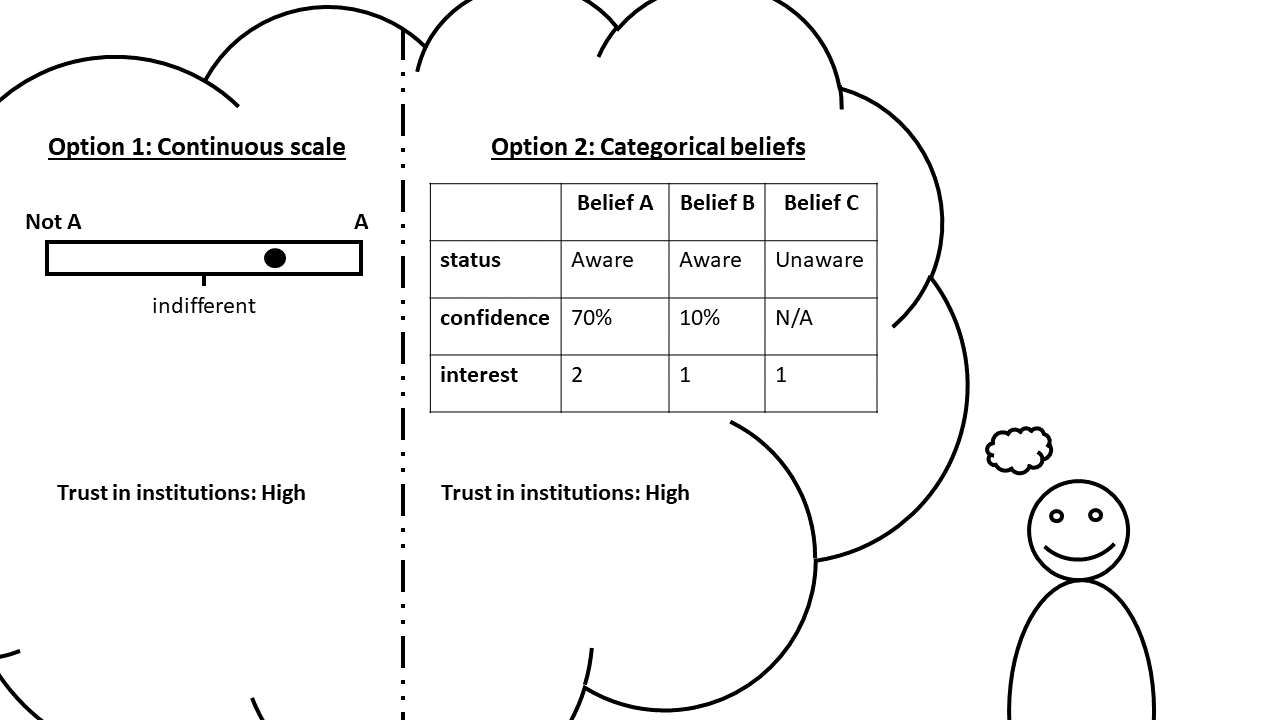
\includegraphics[scale=0.5]{internalstates}
	\centering
	\caption{Two different proposals to model beliefs in the model, depending on the goal of the spreader.}
	\label{img:beliefs}
\end{figure}



\subsection{Model Psuedocode}
This section contains pseudocode for model initialisation and one timestep, as well as suggestions for some lower-level processes. The latter should really only be taken as suggestions that I've included because they might clarify my thinking - their actual implementation is going to be case and interest specific - so they're not based on too much and should be treated accordingly. \\

I am ambigious about what a timestep represents (a day? an hour? a month?) and this is very much deliberate. To me, the length represented by a timestep would really depend on the case you want to model and it makes little sense to define it now. If you're modelling disinformation that has been introduced in a crisis setting, people are probably posting information in quick succession and reacting to it in a similar matter, so a timestep could be 15 minutes. Clearly, governments and platforms will not be able to respond so quickly and you can compensate for this by reducing their effectiveness. On the flipside, a disinformation campaign aimed at creating societal polarisation takes place over the course of years, so you could use a timestep of a day or even a week. COVID-related disinformation probably sits somewhere in the middle of these examples. The current conceptualisation of the model should give you enough flexibility to end up with a sensible model as long as a timestep lies between minutes and months.  \\ 

\begin{algorithm}[H]
	\SetAlgoLined
	\SetKwInOut{Input}{input}\
	\caption{Pseudocode for model initialisation}
	\Input{Model Parameters: Network properties \& size, Belief representation, Spreader strategy, Spreader belief(s), Spreader budget, Platform effectiveness, Government effectiveness, Government strategy, Government belief, Governmet budget}
	
	\BlankLine
	\BlankLine
	
	initialize\_individuals(Belief representation)\;	
	initialize\_Spreader(Spreader strategy, Spreader beliefs)\;
	initialize\_Platform(Platform effectiveness)\;
	initialize\_Government(Government effectiveness, Government strategy, Government belief)\;
	
	\BlankLine
	\BlankLine
	
	initialize\_online\_network(Network properties, size)\;
	initialize\_offline\_network(Network properties, size)\;
	
	spreader.place\_bots(Spreader strategy, Spreader belief, Spreader budget)\;
	
	
\end{algorithm}

\begin{algorithm}[H]
	\SetAlgoLined
	\ForEach{individual $\in individuals$}{
		online\_input = observe.online\_connections()\;
		offline\_input = observe.offline\_connections()\;
		individual.adjust\_belief(online\_input, offline\_input)\;
		individual.evaluate\_online\_relations(online\_input)\;
		individual.evaluate\_offline\_relations(offline\_input)\;	
	}
	\BlankLine
	\BlankLine
	\tcc{Now the ``strategic actors'' observe the environment and take action accordingly.}
	\If{platform.detect\_bots() == TRUE}{platform.remove\_bot\_group()\;}
	\eIf{government.campaign\_detected == TRUE}
		{government.use\_bots(strategy)\;}
		{government.monitor\_for\_campaigns()\;}
	
	spreader.use\_bots(strategy)\;
	
	\BlankLine
	\BlankLine
	
	\ForEach{individual $\in individuals$}
		{individual.post\_online()\;
		 individual.talk\_offline()\;}
	 \For{bot $\in bots$}
	 	{bot.post\_as\_instructed()\;}
	\caption{Pseudocode for 1 timestep of the ABM}
\end{algorithm}



\begin{algorithm}[H]
	\SetAlgoLined
	\ForEach{online\_connection $\in$ online\_connections}{
		\If{if expressed\_belief == A}{ expressed\_A\_online =+ 1\;}
		\If{if expressed\_belief == B}{ expressed\_B\_online =+ 1\;}
		\If{if expressed\_belief == C}{ expressed\_C\_online =+ 1\;}}
	
	\BlankLine
	\BlankLine
	\tcc{Repeat for offline beliefs}
	
	\BlankLine
	\BlankLine
		
	\ForEach{belief $\in$ [A, B, C]}
		{\If{belief.status == unaware AND (expressed\_belief\_online > 1 OR expressed\_belief\_offline > 1 }{belief.status = aware\;}
		
		\BlankLine
		
	
		belief.confidence = ( expressed\_belief\_online + expressed\_belief\_offline)/ total\_connections\;
	}
		\BlankLine
		\BlankLine
		\tcc{For sharing a belief, an individual has to choose one, based on their confidence and the interest in the belief}
		
		\BlankLine
		\BlankLine
		
		p\_A = A.confidence * A.interest\;
		p\_B = p\_A + B.confidence * B.interest\;
		p\_C = p\_B + C.confidence * C.interest\;
		
		p = random\_number(200)\;
		\uIf{0 $=< p <$ p\_A}{express.belief(A)\;}
		\uElseIf{p\_A $=< p <$ p\_B}{express.belief(B)\;}
		\uElseIf{p\_B $=< p <$ p\_C}{express.belief(C)\;}
		\Else{\tcc{Do Nothing}}
		
	
	
	\caption{Pseudocode for an individual updating and sharing their belief(s) using categorical beliefs}
\end{algorithm}








\subsection{Variables and possible RQs}
Currently the model has a lot of undefined variables. Some of them are clear ``policy levers'' that can be experimented with, such as the effectiveness of governments and platforms in detecting disinformation campaigns or individual's trust in government. Others are context-dependent, such as the conceptualisation of beliefs as well as the topology and overlap of the networks. Some variables, such as the change in an individual's belief based on the beliefs expressed in their networks, and the likelihood of breaking ties with someone probably just need to be assumed on a ``educated guess'' basis in the first implementations of this model. I would recommend extensive sensitivity analysis for these variables - if it turns out their role in the model behaviour is significant, it is an option to expand the current conceptualisation in more complex, stand-alone mechanisms.\\

Below, I've provided some suggestions for research questions that I believe can be investigated with this model. What variables with be your levers, and which ones become constants (after sensitivity analysis) will depend on the question.


\begin{itemize}
	\item How does the network topology (of the online and offline networks) influence the succes of a disinformation campaign?
	\item How does the level of overlap between the two networks influence the succes of a disinformation campaign?
	\item How sensitive are the outcomes of the model to different conceptualisations of opinion change? (For inspiration look at \cite{Flache2017}).
	\item Can you cause polarisation in the offline network?
	\item Is the counter-campaign by a government sensitive to the strategy chosen by the spreader?
\end{itemize}

\section{Who else is working on this?}
At TPM, Natalia Kodenko is also working on disinformation from a more qualitative/humanities perspective. Lavina Marin is also supposedly working on the topic or has done so in the past - however I have not spoken to her about this. 
While I was at TPM there was talk of starting a Disinformation Lab. The first steps to do so were taken by me, Natalia and Thomas Baar. (Wolter Pieters became involved at a later stage as I was leaving). We have also been collaborating with an organisation called DROG with their ADTAC programme. Natalia and I designed an experiment/summerschool with them and they rreviously organised a workshop with the TU.

\bibliographystyle{apacite}
\bibliography{RP_lib}
	
\end{document}


%lit review

%conceptual model